\begin{figure*}[t]
\centering
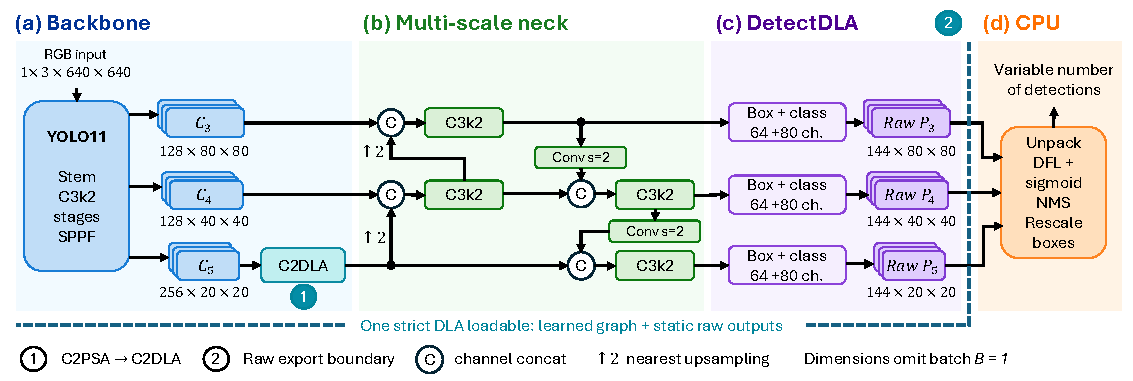
\includegraphics[width=0.95\textwidth]{figures/architecture_overview.pdf}
\caption{\textbf{YOLO11-DLA architecture.} Backbone scales feed the neck and box/class
 towers at strides 8, 16, and 32. Markers 1 and 2 identify C2DLA and the raw-output
 boundary. The learned graph forms one DLA loadable; unpacking and post-processing
 remain on CPU. Preprocessing and input packing precede the graph.}
\label{fig:boundary}
\end{figure*}
